\chapter{Technische Grundlagen}
	Nachstehend werden die technischen Grundlagen erläutert und es wird kurz auf diese eingegangen. Dabei wird mit den Entwicklungsumgebungen begonnen.

\section{Unity}
Bei Unity handelt es sich um eine Entwicklungs- und Laufzeitumgebung, mit deren Hilfe graphisch aufwändige Projekte umgesetzt werden können. Dazu gehören unter anderem Videospiele, aber auch Lernprogramme oder Apps können damit umgesetzt werden. Dazu können in Unity 3D-Projekte, aber auch 2D beziehungsweise 2,5D Projekte umgesetzt werden(Dabei handelt es sich um eine Mischung von 2D und 3D Spielen). Dank Unity sind diese Projekte nach der Entwicklung plattformübergreifend einsetzbar.\footnote{vgl. Unity3D \cite{unity1} (2017)} Die Entwicklungsumgebung teilt sich dabei in verschiedene Bereiche auf. Diese sind dabei an einen 3D-Editor angelegt.

Das „Scene” Fenster ist in den Standardeinstellungen in der Mitte des Bildschirms zu sehen(Siehe Abbildung \ref{scene} )\footnote{vgl. Unity3D \cite{unity2} (2017)}.

\begin{figure}[htbp]
\centering 
\label{scene}
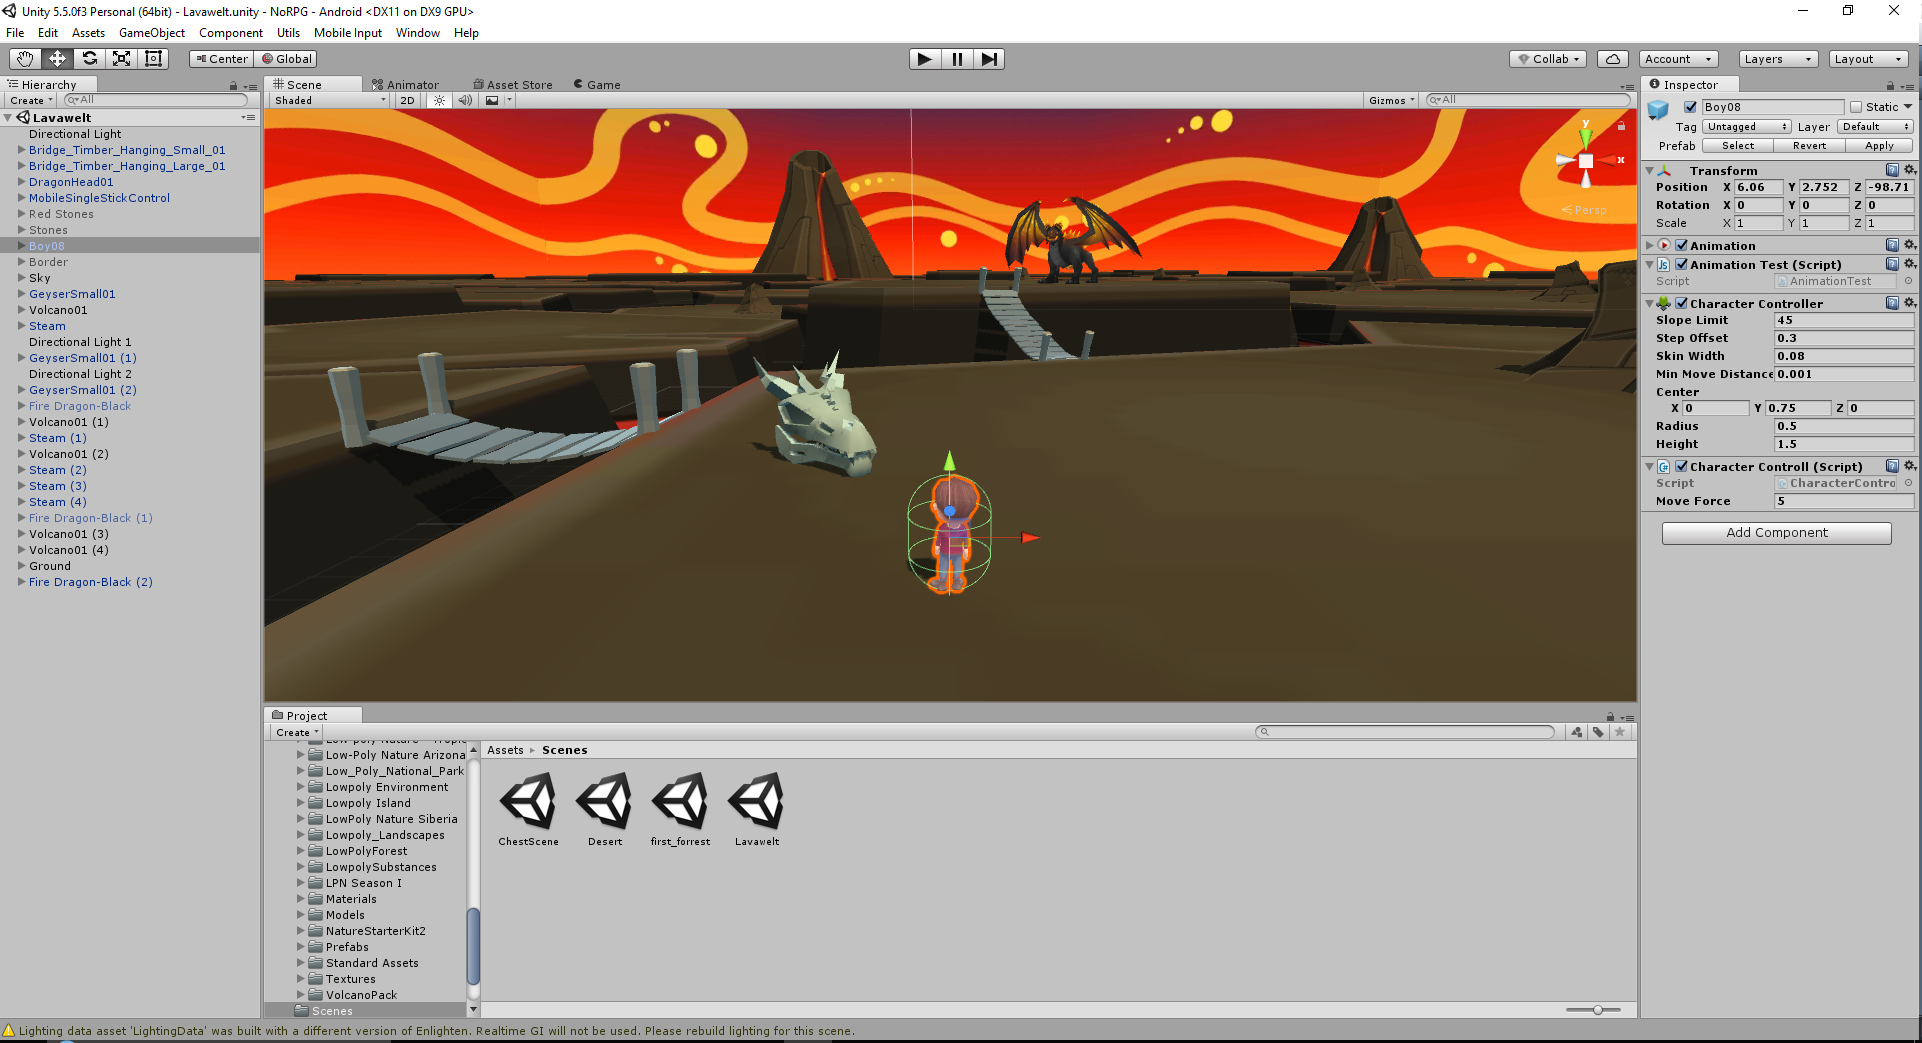
\includegraphics[width=0.9\textwidth]{pics/unity3d_ui.png}
\caption{Darstellung von Tablemappings}
\end{figure}

Hier wird immer die aktuelle Szene dargestellt. Darüber hinaus kann hier mit Objekten der Szene interagiert werden, um diese zu verändern, zum Beispiel an eine andere Stelle platzieren oder zu skalieren.

Wird ein Objekt in diesem Fenster ausgewählt, befinden sich im Bereich „Inspector” zusätzliche Einstellmöglichkeiten\footnote{vgl. Unity3D \cite{unity3} (2017)}.
Diese variieren je nach gewähltem Objekt. Auch hier können die Position oder die Skalierung eines Objektes verändert werden, allerdings werden hier auch darüber hinausgehende Eigenschaften der Objekte verändert. Dazu zählen die visuellen sowie die physischen Eigenschaften der Objekte. 

Ein weiterer Weg, ein Objekt auszuwählen, ist das markieren im „Hierarchy” Fenster\footnote{vgl. Unity3D \cite{unity4} (2017)}. 
In diesem Fenster werden alle Objekte der aktuellen Szene aufgelistet. Dabei wird zwischen unterschiedlichen Ebenen unterschieden, so dass genau gesehen werden kann welche Objekte zusammengehören. 

Um alle Dateien zu sehen, die zu einem Projekt gehören, gibt es das „Project” Fenster\footnote{vgl. Unity3D \cite{unity5} (2017)}. Die Dateien werden dabei nach der vorliegenden Ordnerstruktur angezeigt. In diesem Fenster können Ordner, sowie andere Dateien erstellt werden.

Ein weiteres wichtiges Fenster ist das „Game” Fenster\footnote{vgl. Unity3D \cite{unity6} (2017)}. Hier kann das fertige Projekt angesehen werden. Dazu gibt es oben in der Mitte der Benutzeroberfläche, ein Start, Pause und Vorlauf Button. Mit Hilfe derer kann das Programm, bevor es auf der Zielplattform abgespielt wird, in der Entwicklungsumgebung gerendert werden. Der Code wird von Unity JustIn-Time (JIT) kompiliert, und anschließend auf Mono oder dem Microsoft .NET Framework ausgeführt. Der Code steht in sogenannten Skripten, die in C\#, UnitySkript (ähnlich JavaScript) oder Boo geschrieben sind.

Wenn während der Laufzeit oder im Vorfeld beim Kompilieren ein Fehler auftritt, wird dieser im „Console” Fenster ausgegeben. Darüber hinaus werden hier Meldungen angezeigt, die explizit in den Skripten programmiert wurden.
Damit es zu keinen Fehlern kommt, gibt es in Unity Tests, die eine Szene auf Korrektheit prüft. Die sogenannten Integrationstest simulieren eine Szene, damit verschiedene Objekte auf ihre Eigenschaften geprüft werden können. 

Nachdem nun die Benutzeroberfläche ausführlich erklärt wurde, wird nun auf die Begriffe Prefabs und Skripte eingegangen, da diese Essentiell für den Umgenag mit Unity sind.

\textbf{Prefabs}

Bei Prefabs handelt es sich um fertige Objekte, die in Szenen verwendet werden können\footnote{vgl. Unity3D \cite{unity7} (2017)}. Diese können dabei als Vorlage gesehen werden, damit nicht jedes Objekt mit gleichen Eigenschaften erneut erstellt werden müssen. 

\textbf{Skripte}

In Skripten befindet sich die Logik von Objekten\footnote{vgl. Unity3D \cite{unity8} (2017)}. Ein Beispiel dafür ist das Öffnen einer Truhe. Wenn der Benutzer die Truhe anklickt und öffnen will, steht in einem Skript, was die Truhe zu tun hat. In diesem Beispiel also, das sie sich öffnen soll. 

Diese Logik kann mithilfe einer Entwicklungsumgebung angepasst werden. Die dazu geeignete Entwicklungsumgebung wird bei der Installation von Unity mitgeliefert. Dabei handelt es sich um Microsoft Visual Studio.

\section{Visual Studio}

Mit Microsoft Visual Studio ist es möglich in verschiedenen Programmiersprachen zu programmieren\footnote{vgl. Microsoft \cite{microsoft1} (2015)}.
Bei der Installation von Unity wird dieses dabei zusätzlich installiert. Dadurch können die Skripte aus Unity in Visual Studio geöffnet und bearbeitet werden. Zusätzlich zu Visual Studio werden auch verschiedene Plug-Ins für die IDE installiert. Dabei handelt es sich unter anderem um eine ausführliche Dokumentation von allen in Unity zur Verfügung stehenden Methoden und Klassen sowie um Testtools, um verschiedene Tests auszuführen. 

\section{C Sharp}

C\# (gesprochen C Sharp) ist eine Programmiersprache welche von Microsoft entwickelt wurde. Sie wurde zusammen mit „.NET 1.0” 2002 in der Version 1 veröffentlicht und ist mittlerweile in Version 6 verfügbar.\footnote{vgl. Microsoft \cite{microsoft2} (2015)} 

C\# orientiert sich dabei an den Programmiersprachen C, C++, Java, Delphi und Haskell und nutzt deren grundlegenden Konzepte. Aufgrund der Ähnlichkeit zu diesen Sprachen handelt es sich bei C\# ebenfalls um eine Objektorientierte Sprache. 

Nachfolgend wird nun auf die Grundlegenden Konventionen eingegangen, denen C\# zugrunde liegen. Danach wird auf die Verwendung in Unity Skripten eingegangen.

\subsection{Allgemeiner aufbau C\#}

Der allgemeine Aufbau von C\# wird hier am Beispiel von einem Hello World Programm in Listing \ref{lst:c_helloworld} dargestellt. 

Dabei ist in Zeile eins ein Text zu sehen. Vor diesem stehen zwei Slashes. Damit wird der Text als Kommentar gekennzeichnet. Daruch wird dieser Abschnitt vom Compiler beim Compilieren ignoriert. In Zeile zwei wird das Schlüsselwort „using” gefolgt von einem Namen, in diesem Fall „System”, genutzt. Dieses dient dazu um das Package System in dem Programm zu nutzen.

\begin{scriptsize}
\lstset{
	float,
	caption=Hello World in C\#, 
	language=[Sharp]C, 
	frame=single,  
	showstringspaces=false, 
	showspaces=false, 
	numbers=left, 
	captionpos=b, 
	belowcaptionskip=4pt,
	basicstyle=\ttfamily
} 

\begin{lstlisting}[label=lst:c_helloworld]
// A Hello World! program in C#.
using System;
namespace HelloWorld
{
    class Hello 
    {
        static void Main() 
        {
            Console.WriteLine("Hello World!");

            // Keep the console window open in debug mode.
            Console.WriteLine("Press any key to exit.");
            Console.ReadKey();
        }
    }
}
\end{lstlisting}
\end{scriptsize}

Als nächstes wird ein Namespace definiert. Innerhalb von diesem eine Klasse namens „Hello”. Innerhalb von dieser wiederum befindet sich der auszuführende Code.

Dieser steht in einer Methode, die in Zeile sieben definiert wird. Bei dieser Methode handelt es sich um die Main() Methode. Diese wird beim Programmstart immer zuerst ausgeführt. In dieser Methode gibt es vier Zeilen Code, darunter ein Kommentar(in Zeile elf). Bei den anderen drei Zeilen handelt es sich um Konsolenausgaben bzw. Konsoleneingaben. Die Zeilen neun und zwölf geben jeweils Text auf der Konsole aus. In Zeile 13 wird dagegen ein Zeichen eingelesen, welches vom Benutzer eingegeben wird.

\subsection{Unity Skripte}

Die in Unity verwendeten C\# Skripts erben standardmäßig von der Klasse Mono-Behaviour wie in Listing \ref{lst:unity3Dc} zu sehen. Diese Vererbung sorgt dafür, dass jede Klasse verschiedene Methoden zur Verfügung hat. Dazu zählt eine Start-Methode, die beim Laden eines Objekts mit dem Skript ausgeführt wird und eine Update-Methode, die bei jeder Frameaktualisierung ausgeführt wird. Des Weiteren können weitere Methoden genutzt werden. Außerdem sorgt die MonoBehavior Vererbung dafür, dass diese Skripte mit Objekten in Unity verknüpft werden können.

\begin{scriptsize}
\lstset{
	float,
	caption=Aufbau eines Unity Skriptes, 
	language=[Sharp]C, 	
	frame=single,  
	showstringspaces=false, 
	showspaces=false, 
	numbers=left, 
	captionpos=b, 
	belowcaptionskip=4pt,
	basicstyle=\ttfamily
} 

\begin{lstlisting}[label=lst:unity3Dc]
using System.Collections;
using System.Collections.Generic;
using UnityEngine;

public class test : MonoBehaviour {

	// Use this for initialization
	void Start () {
		
	}
	
	// Update is called once per frame
	void Update () {
		
	}
}
\end{lstlisting}
\end{scriptsize}	

\section{SQL}

SQL ist im Allgemeinen als Akronym für „Structured Query Language“ gesehen, obwohl SQL eine eigenständige Bezeichnung ist.\footnote{vgl. Beaulieu, Alan\cite{sql1} (2009) S.8} SQL wird dazu verwendet, um Daten in relationalen Datenbanken zu bearbeiten, abzufragen und anzulegen.\footnote{vgl. Beaulieu, Alan\cite{sql1} (2009) S.IX} Die Syntax von SQL orientiert sich an der englischen Sprache. Um unabhängig von einem Datenbanksystem zu sein, wird häufig SQL verwendet, da SQL von vielen Datenbanken unterstützt wird.\footnote{vgl. Adams, Ralf\cite{sql2} (2012) S. 63 ff.}